\documentclass[11pt]{article}
\usepackage[a4paper,margin=1in]{geometry}
\usepackage[T1]{fontenc}
\IfFileExists{lmodern.sty}{\usepackage{lmodern}}{\usepackage{mathptmx}}
\usepackage{microtype}
\usepackage{amsmath,amssymb}
\usepackage{booktabs}
\usepackage{graphicx}
\usepackage{xcolor}
\usepackage[numbers,sort&compress]{natbib}
\usepackage[colorlinks=true,linkcolor=blue!50!black,citecolor=blue!50!black,urlcolor=blue!50!black]{hyperref}
\usepackage{enumitem}
\setlist{nosep,leftmargin=*}

\newcommand{\code}[1]{\texttt{#1}}
\newcommand{\repo}{\href{https://github.com/Riks1/WPL-Final}{\code{github.com/Riks1/WPL-Final}}}

\title{Win Probability for the Women's Premier League:\\
A Reproducible Baseline, As-Of Player Ratings,\\ and a Pre-Specified Null Result}
\author{Haarika\\ \small Code, data hashes and reports: \repo}
\date{November 2026}

\begin{document}
\maketitle

\begin{abstract}
We build and evaluate win-probability models for the Women's Premier League (WPL), a T20 franchise
competition with only 22 matches a season. Every model is scored out of sample with rolling-origin
season folds, per-match log-loss, and a paired bootstrap over matches, and every deployment decision
follows a rule fixed before the final run. For live (in-match) prediction, a five-parameter par-score
model, a Duckworth--Lewis-style resource curve with negative binomial noise, beats the base rate by
$0.175$ log-loss [$0.059$, $0.286$] on 66 held-out matches, and neither logistic regression nor a random
forest beats it. For pre-match prediction we construct ball-level, as-of, empirical Bayes player
ratings from 799{,}502 deliveries of women's T20 cricket and aggregate them into an XI-strength margin.
Under a pre-specified rule, this model does \emph{not} beat the base rate in the WPL: it is worse by
$+0.087$ [$+0.012$, $+0.162$]. The same features and code improve log-loss by $0.203$ [$0.079$, $0.312$] on
53 India T20Is, a supporting analysis, and an exploratory breakdown traces the WPL failure to a single
22-match training fold. We report the null result as the finding, describe the reproducibility
infrastructure (hash-pinned data snapshots, leakage tests, JSON-only model artefacts), and disclose a
lapse in our pre-registration record.
\end{abstract}

\section{Introduction}

Win-probability models are the backbone of in-play analytics, broadcasting graphics and, increasingly,
team decision support. Women's franchise cricket poses a specific difficulty: the WPL began in 2023 and
plays 22 matches a season, so any model is trained and tested on a few dozen matches, and wide
uncertainty is the norm rather than the exception. In this regime the dominant risk is not
under-fitting but self-deception: leakage between training and test, metrics computed on the wrong
unit, and model choices tuned on the test set.

This report documents the first three stages of a project that treats those risks as the central design
constraint. Our contributions are:
\begin{enumerate}
  \item An evaluation protocol for small-sample sports forecasting: rolling-origin season folds,
        per-match log-loss, paired bootstrap intervals over matches, and deployment rules written down
        before the final run (\S\ref{sec:protocol}).
  \item A live win-probability model built on a parametric par-score curve that beats flexible learners
        on held-out seasons, together with an audit of an earlier version whose reported accuracy was an
        artefact of leakage and a majority-class predictor (\S\ref{sec:live}).
  \item Ball-level, strictly as-of, empirical Bayes player ratings for women's T20 cricket, with
        leakage tests, and an aggregation into a pre-match XI-strength margin (\S\ref{sec:ratings}).
  \item A pre-specified evaluation that rejects deploying those features in the WPL, with supporting and
        exploratory evidence about why (\S\ref{sec:prematch}).
\end{enumerate}
All results in this report are regenerated from the repository by the commands in Appendix~\ref{app:repro}.

\section{Data}\label{sec:data}

\paragraph{Source and snapshots.} Ball-by-ball data come from Cricsheet~\citep{cricsheet}. Every
download is frozen as a zip snapshot, published to a Hugging Face dataset, and registered in git with its
SHA-256; the loader refuses a file whose hash does not match. Stage~1 used a WPL-only snapshot
(\code{wpl\_json\_20261025}, 88 matches); Stages~2--3 use a snapshot of all women's matches
(\code{all\_female\_json\_20261025b}, SHA-256 \code{0f5bb2ac\ldots}).

\paragraph{Tables.} A parser turns each match into tidy tables (matches, innings, deliveries, wickets,
team sheets, replacements) plus entity tables (people, venues, team switches). Table~\ref{tab:data}
summarises the build. A validation pass flags anomalies (e.g.\ overs with seven legal balls, scorer
errors in associate matches); none of the flags falls inside the modelling scope. One awarded match is
excluded. Re-parsing the 88 WPL matches through the Stage~2 parser reproduces the Stage~1 ball table
exactly (zero drift), and the two pipelines give the same base-rate log-loss on the common test set
(0.703 in both Table~\ref{tab:live} and Table~\ref{tab:wpl}).

\begin{table}[t]\centering\small
\caption{The Stage 2 data build (snapshot \code{all\_female\_json\_20261025b}).}\label{tab:data}
\begin{tabular}{lr}\toprule
Matches parsed (20-over women's T20s) & 3{,}508 \\
\quad of which no result / tie / tie decided by super over & 67 / 10 / 23 \\
Main-innings deliveries & 799{,}502 \\
Players / venues & 3{,}418 / 305 \\
Model scope: WPL / India T20Is / Women's T20 Challenge & 88 / 171 / 13 \\
\bottomrule\end{tabular}
\end{table}

\paragraph{Label.} The target is $y=1$ if the team batting first wins. Stage~1 credited a tie decided by
a super over to the super-over winner; Stage~3 scores an unresolved tie as $y=0.5$, which is the correct
probability target for log-loss. No-results have no label and are excluded; the WPL test set contains no
ties under either convention.

\section{Evaluation protocol}\label{sec:protocol}

\paragraph{Folds.} Rolling origin~\citep{tashman2000}: for each test season
$S\in\{2024,2025,2026\}$, models are fitted on seasons before $S$ only. This gives 66 WPL test matches.

\paragraph{Metric.} The headline metric is log-loss, a strictly proper scoring rule~\citep{gneiting2007},
averaged \emph{per match}: in live evaluation a match contributes about 240 ball-level predictions, and
averaging over balls would let long matches dominate. We also report the Brier score~\citep{brier1950},
expected calibration error (ECE, 10 bins), and the calibration slope and intercept~\citep{collins2015,vancalster2019}:
the slope from regressing $y$ on $\operatorname{logit}(p)$ (ideal 1; below 1 means over-confident), the
intercept from the same model with $\operatorname{logit}(p)$ as an offset (ideal 0).

\paragraph{Uncertainty.} 95\% percentile intervals come from 2{,}000 bootstrap resamples of
\emph{matches}~\citep{efrontibshirani1993}, seed 0. Comparisons are paired: every model is scored on the
same resampled matches, so the interval for a difference reflects match-to-match variation once.

\paragraph{Decision rules.} Each stage fixes its rule before its final run. Stage~1 deploys the par-score
model unless a learned model beats it with a paired interval excluding zero. Stage~3 deploys its
primary pre-match model if and only if the upper end of the 95\% interval for
(primary $-$ base rate) is below zero. Stage~1's paired interval on the same 66 matches had a
half-width of about 0.067, so improvements smaller than roughly 0.07 log-loss are not detectable; we
stated this power limit before the run.

\section{Stage 1: live win probability}\label{sec:live}

\paragraph{Par-score model.} Following the resource idea behind Duckworth--Lewis~\citep{duckworth1998,stern2016},
the expected runs still to come with $u$ overs left and $w$ wickets lost are
\begin{equation}
  \mu(u,w) = \frac{r(w)}{b(w)}\bigl(1-e^{-b(w)\,u}\bigr),\qquad
  r(w)=\exp\!\bigl(a_0-e^{t_1}w\bigr),\quad b(w)=\exp(c_0+c_1 w),
\end{equation}
and the runs to come $R$ follow a negative binomial with mean $\mu$ and dispersion $\alpha$. In the second
innings, with $n$ runs needed, $P(\text{bat-first wins}) = P(R\le n-2)+\tfrac12 P(R=n-1)$. In the first
innings, the final total $T=s+R$ is mapped to a win probability through a logistic link fitted on past
matches, $P=\sum_k P(R=k)\,\sigma\!\bigl(a+c\,(s+k-\bar t)/s_t\bigr)$. Terminal states are deterministic.

\paragraph{Results.} Table~\ref{tab:live} compares the par-score model with a constant base rate,
per-innings logistic regression and a random forest, in the spirit of in-play cricket
models~\citep{asif2016}. The par-score model beats the base rate clearly, while the logistic model's interval
reaches zero and the random forest's straddles it; under the Stage~1 rule the par-score model is deployed
(logistic $-$ par-score $=+0.047$ [$-0.023$, $+0.118$]; random forest $-$ par-score $=+0.124$ [$+0.045$, $+0.208$]). Poisson noise is clearly worse than negative binomial:
run scoring is overdispersed. Post-hoc calibrators~\citep{guo2017} fitted on earlier seasons did not help:
Platt scaling ($+0.060$ [$+0.006$, $+0.116$]) and isotonic regression ($+0.082$ [$+0.023$, $+0.144$]) made
the par-score model worse, and temperature scaling changed nothing. Figure~\ref{fig:rel1} shows
reliability by innings.

\begin{table}[t]\centering\footnotesize\setlength{\tabcolsep}{4pt}
\caption{Stage 1 live models on 66 held-out WPL matches (2024--2026). Per-match log-loss and Brier;
$\Delta$ is paired against the base rate.}\label{tab:live}
\begin{tabular}{lcccc}\toprule
Model & Log-loss [95\% CI] & $\Delta$ vs base [95\% CI] & Brier & ECE\\\midrule
Base rate (constant) & 0.703 [0.633, 0.770] & 0 & 0.254 & 0.127\\
\textbf{Par-score: DLS curve + negative binomial} & \textbf{0.528} [0.428, 0.633] & $-$0.175 [$-$0.286, $-$0.059] & 0.179 & 0.064\\
Par-score: DLS curve + Poisson & 0.663 [0.472, 0.874] & $-$0.040 [$-$0.235, $+$0.178] & 0.190 & 0.107\\
Logistic regression, per innings & 0.575 [0.453, 0.717] & $-$0.128 [$-$0.243, $+$0.002] & 0.190 & 0.079\\
Random forest, per innings & 0.652 [0.512, 0.814] & $-$0.050 [$-$0.185, $+$0.101] & 0.208 & 0.108\\
\bottomrule\end{tabular}
\end{table}

\begin{figure}[t]\centering
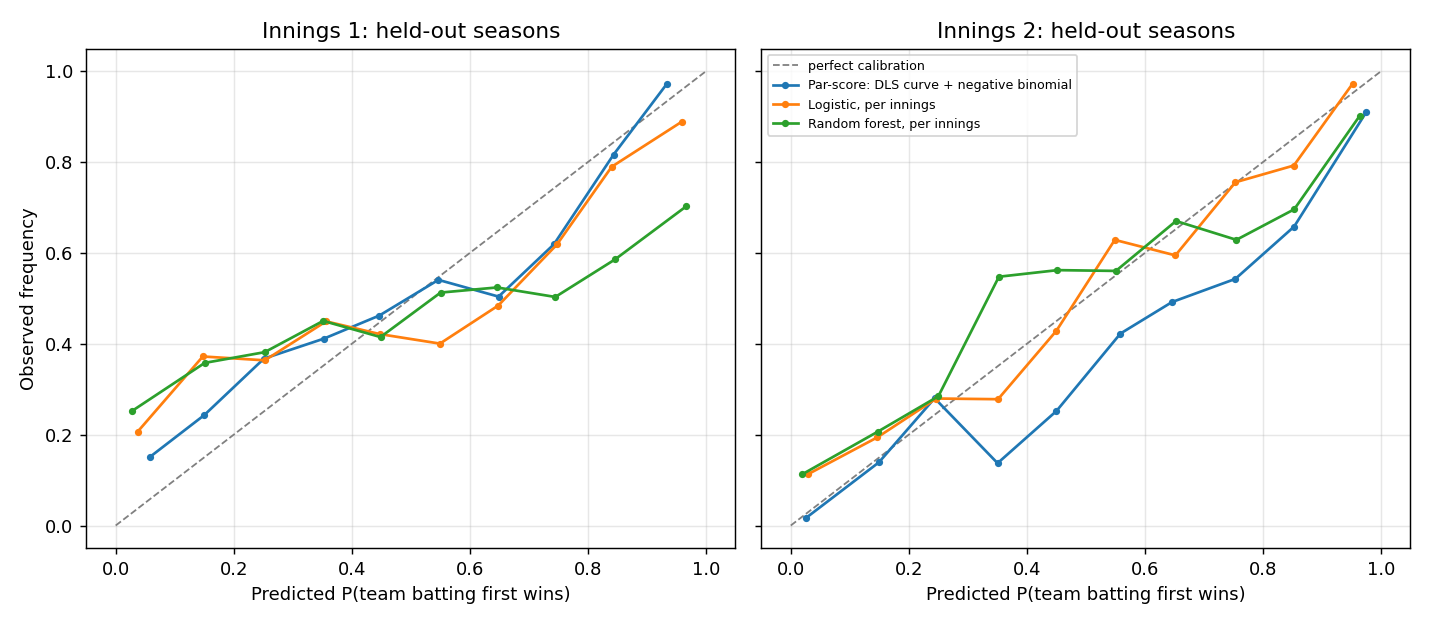
\includegraphics[width=\linewidth]{reliability_stage1.png}
\caption{Stage 1 reliability of the live models on held-out seasons, by innings.}\label{fig:rel1}
\end{figure}

\paragraph{Pre-match.} A post-toss model using recent form, head-to-head record and the toss scored
\emph{worse} than the base rate ($+0.066$ [$+0.001$, $+0.135$]), so the pre-match endpoint serves the base
rate and says so in its response. This motivates Stage~3: team-level history is a weak proxy for who is
actually playing.

\paragraph{Audit of the earlier version.} Stage~1 began as an audit of an earlier model and is reproducible
by script. Its reported pre-match accuracy of 73.8\% equalled the majority-class rate (the model predicted
one class for every match); its live model never saw the target, because \code{target} and
\code{runs\_needed} were zero on every training row; its reported live log-loss leaked, because
cross-validation split ball rows so that every match was in both training and validation; and the
deployed model received unscaled inputs, giving 51--53\% for won and lost chases alike.

\section{Stage 3: as-of player ratings}\label{sec:ratings}

The goal is a per-player measure of batting and bowling quality that, for a match on date $d$, uses only
deliveries dated before $d$. We rate four components per player: batting runs per ball, batting
dismissal per ball, bowling runs conceded per ball and bowling wickets per ball. The full specification
is \code{docs/stage3/RATINGS\_SPEC.md}.

\paragraph{Expected outcome per ball.} For ball $i$ and component $c$, the expectation is
\begin{equation}
  e_i^c = m^c_{\text{cell}(i)} + \mathbb 1[c\in\text{runs}]\,v_{\text{venue}(i)} + \theta^{c'}_{\text{opp}(i)},
\end{equation}
where the cell is (competition, phase of innings, wickets lost, innings), $m$ is its time-decayed mean shrunk
towards a pooled cell (prior strength $k_{\text{cell}}=500$ balls), which is in turn shrunk towards the overall
mean ($k_{\text{pool}}=2{,}000$); $v$ is a venue run effect shrunk towards zero ($k_{\text{venue}}=1{,}000$);
and $\theta^{c'}_{\text{opp}}$ is the opponent's matching as-of rating (a batter's expectation includes the
bowler's runs-conceded rating, and vice versa). Ratings are deviations from the cell average, so the
opponent's rating is added as is.

\paragraph{Empirical Bayes update.} With residuals $r_i=y_i^c-e_i^c$ and weights
$w_i=2^{-(d-d_i)/h}$ for a half-life of $h$ years, player $p$'s rating and its uncertainty are
\begin{equation}
  \theta^c_p(d) = \frac{\sum_{i\in p,\,d_i<d} w_i r_i + k_c\,\mu_{0,c}}{\sum_{i\in p,\,d_i<d} w_i + k_c},
  \qquad
  \operatorname{sd}\bigl(\theta^c_p\bigr)=\sqrt{\frac{\sigma_c^2}{\sum w_i + k_c}},
\end{equation}
the posterior mean of a normal model with prior mean $\mu_{0,c}$ and prior strength $k_c$
balls~\citep{efronmorris1975}. A two-pass procedure estimates the priors on balls before 2024-01-01 only:
pass~1 computes residuals; $\mu_{0,c}$ is the mean residual over players' first 60 balls (a debutant prior);
$\sigma_c^2$ is the residual variance; and $k_c=\sigma_c^2/\tau_c^2$, where the between-player variance
$\tau_c^2$ is estimated by the method of moments. The build walks match dates in order and
records, predicts, then learns, so matches on the same day never see each other. Table~\ref{tab:ratings}
gives the fitted values: the run components shrink lightly ($k\approx 75$ balls) while the bowling-wicket
component needs about 2{,}100 balls of evidence to move halfway from the prior, which says wicket-taking
skill is hard to distinguish from luck at the ball level.

\begin{table}[t]\centering\small
\caption{Ratings hyperparameters, all estimated on balls before 2024-01-01. Top: half-life $h$ chosen by one-step-ahead MSE of batting runs per ball on 2022--2023 (166,369 balls). Bottom: empirical Bayes prior mean $\mu_0$ (debutant prior), residual variance $\sigma^2$ and prior strength $k=\sigma^2/\tau^2$ (in balls).}\label{tab:ratings}
\begin{tabular}{lcccc}\toprule
Half-life $h$ (years) & 1 & 2 & 4 & $\infty$\\
MSE & 1.72912 & 1.72775 & \textbf{1.72738} & 1.72779\\\bottomrule\end{tabular}

\vspace{6pt}
\begin{tabular}{lccc}\toprule
Component & $\mu_0$ & $\sigma^2$ & $k$\\\midrule
Batting runs & $-$0.1221 & 1.6984 & 73.3\\
Batting dismissal & $+$0.0102 & 0.0483 & 129.2\\
Bowling runs & $+$0.0387 & 1.6552 & 77.2\\
Bowling wicket & $-$0.0024 & 0.0434 & 2123.5\\
\bottomrule\end{tabular}
\end{table}


\paragraph{Leakage tests.} The test suite checks that perturbing any future delivery leaves every earlier
rating unchanged, that same-day matches are isolated, that a debutant receives exactly the prior, that the
decay halves a ball's weight after $h$ years, and that the build is deterministic (the content hash of the
ratings table, \code{1e5c4bd4\ldots}, reproduced exactly after a rebuild from scratch). Two leaks were caught
by these tests during development and fixed before any evaluation: $\sigma^2$ computed from the full data,
and first-day matches predicted from their own outcomes.

\paragraph{XI strength.} For each team's toss XI (the team sheet minus later replacements), batting shares
$s_j$ come from pre-2024 average balls faced by batting position, with the XI ordered by as-of mean
position; bowling shares $q_j$ come from as-of balls bowled per match, capped at 24 of 120. With
$\lambda=18.99$ runs per wicket (pre-2024),
\begin{equation}
  V = 120\sum_j s_j\bigl(\theta^{\text{bat\_runs}}_j-\lambda\,\theta^{\text{bat\_dis}}_j\bigr)
    + 120\sum_j q_j\bigl(\lambda\,\theta^{\text{bowl\_wkt}}_j-\theta^{\text{bowl\_runs}}_j\bigr),
\end{equation}
and \code{xi\_margin} $=V_{\text{bat first}}-V_{\text{chase}}$, in runs. A venue prior,
\code{venue\_bf\_prior}, is the as-of share of matches at the venue won batting first, shrunk towards the
pooled rate with a prior of 20 matches.

\paragraph{Validation without outcomes.} Before any test-season result was scored we checked coverage and
face validity only. The share of WPL XI slots with at least 60 legal balls of history was 0.81, 0.88, 0.86
and 0.93 for 2023--2026. Season-end rankings were stable (Spearman 0.78--0.97 between consecutive seasons,
inflated somewhat by overlapping data under $h=4$). The best-economy lists are led every season by
established international bowlers (e.g.\ M~Kapp, S~Ecclestone, S~Ismail), with a few small-sample entries
(e.g.\ L~Harris's 2023 batting rating) that the shrinkage limits but does not remove.

\section{Stage 3: pre-specified pre-match evaluation}\label{sec:prematch}

\paragraph{Design.} The question was fixed in advance: do XI-strength features improve the post-toss
probability over the base rate? The primary model is a standardised logistic regression
(\code{C}$=1.0$, no tuning) on \code{xi\_margin} and the toss, trained on WPL seasons only. Two secondary
models are reported but cannot earn deployment: S1 adds \code{venue\_bf\_prior}, and S2 uses ratings with
no time decay. India T20Is (training on India T20Is before each test season) form a supporting analysis
that never decides. Hyperparameters were fixed on pre-2024 balls before any test outcome was scored.

\begin{table}[t]\centering\footnotesize\setlength{\tabcolsep}{4pt}
\caption{Pre-match evaluation, WPL (66 test matches, 2024--2026). This comparison decides deployment.}\label{tab:wpl}
\begin{tabular}{lccccccc}\toprule
Model & Log-loss [95\% CI] & $\Delta$ vs base [95\% CI] & Brier & ECE & Cal.\ slope & Cal.\ int. & Acc.\\\midrule
Base rate & 0.703 [0.633, 0.770] & 0 & 0.254 & 0.116 & $-$1.71 & $+$0.23 & 0.576\\
Primary & 0.789 [0.681, 0.901] & $+$0.087 [$+$0.012, $+$0.162] & 0.283 & 0.173 & $-$0.79 & $+$0.19 & 0.530\\
S1 ($+$venue prior) & 0.826 [0.709, 0.942] & $+$0.123 [$+$0.055, $+$0.197] & 0.300 & 0.198 & $-$1.46 & $+$0.26 & 0.530\\
S2 ($h=\infty$) & 0.790 [0.682, 0.903] & $+$0.088 [$+$0.014, $+$0.162] & 0.283 & 0.131 & $-$0.81 & $+$0.19 & 0.530\\
\bottomrule\end{tabular}
\end{table}

\paragraph{Verdict.} Table~\ref{tab:wpl}: the primary model is worse than the base rate by $+0.087$
[$+0.012$, $+0.162$]. The whole interval is above zero, so the base rate remains deployed. S1 is worse
still, and S2 matches the primary, so neither the venue prior nor the choice of half-life rescues the
result. The primary's calibration slope is negative: across the 66 matches its favourites lost more often
than its underdogs (Figure~\ref{fig:rel3}).

\begin{table}[t]\centering\footnotesize\setlength{\tabcolsep}{4pt}
\caption{Supporting analysis, India T20Is (53 test matches, 2024--2026; one no-result excluded). Never decides deployment. $^\dagger$The base rate is almost constant ($\approx 0.48$), so its calibration slope is not estimable in any useful sense.}\label{tab:india}
\begin{tabular}{lccccccc}\toprule
Model & Log-loss [95\% CI] & $\Delta$ vs base [95\% CI] & Brier & ECE & Cal.\ slope & Cal.\ int. & Acc.\\\midrule
Base rate & 0.694 [0.681, 0.706] & 0 & 0.250 & 0.015 & $-$16.12$^\dagger$ & $+$0.06 & 0.509\\
Primary & 0.491 [0.380, 0.611] & $-$0.203 [$-$0.312, $-$0.079] & 0.166 & 0.164 & $+$1.15 & $+$0.03 & 0.717\\
S1 ($+$venue prior) & 0.510 [0.393, 0.643] & $-$0.184 [$-$0.302, $-$0.050] & 0.172 & 0.127 & $+$1.05 & $-$0.11 & 0.717\\
S2 ($h=\infty$) & 0.493 [0.387, 0.607] & $-$0.201 [$-$0.306, $-$0.085] & 0.165 & 0.133 & $+$1.26 & $+$0.02 & 0.698\\
\bottomrule\end{tabular}
\end{table}

\paragraph{Supporting evidence.} On India T20Is (Table~\ref{tab:india}) the same features and code improve
log-loss by $0.203$ [$0.079$, $0.312$], with a calibration slope near one and accuracy of 0.72 against 0.51.
The ratings therefore carry real information about match outcomes. Two caveats keep this from being a
headline: the base rate there is close to 0.5, a weak baseline, and India's fixtures include large strength
gaps that are easy to call.

\begin{figure}[t]\centering
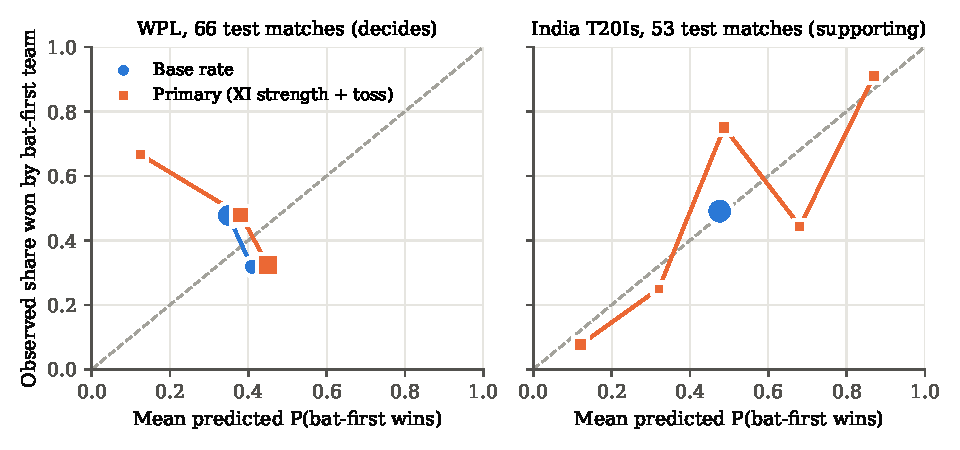
\includegraphics[width=\linewidth]{reliability_stage3.pdf}
\caption{Reliability of the pre-match predictions on the test seasons (5 equal-width bins; marker area
proportional to the number of matches). Left: in the WPL the primary's lowest bin (predicted $\approx 0.13$)
was won by the team batting first two times in three. Right: on India T20Is the primary tracks the diagonal.}\label{fig:rel3}
\end{figure}

\begin{table}[t]\centering\small
\caption{Exploratory, computed after the results were committed; it cannot change the verdict. Per fold: training size, the fitted primary coefficients (per standard deviation of the feature) and the per-match log-loss of the base rate and the primary on that test season.}\label{tab:folds}
\begin{tabular}{lccccccc}\toprule
Data & Test season & $n_{\text{train}}$ & $\beta_{\text{xi}}$ & $\beta_{\text{toss}}$ & $n_{\text{test}}$ & LL base & LL primary\\\midrule
WPL & 2024 & 22 & $-$0.32 & $-$0.90 & 22 & 0.764 & 1.008\\
WPL & 2025 & 44 & $+$0.07 & $-$0.13 & 22 & 0.643 & 0.652\\
WPL & 2026 & 66 & $+$0.09 & $-$0.02 & 22 & 0.701 & 0.708\\
\multicolumn{8}{l}{\quad WPL, test seasons: stronger XI won 0.576 of 66 matches; mean $|\texttt{xi\_margin}|$ = 9.7 runs}\\\midrule
India T20I & 2024 & 113 & $+$1.12 & $+$0.20 & 20 & 0.690 & 0.498\\
India T20I & 2025 & 133 & $+$1.19 & $+$0.21 & 10 & 0.695 & 0.450\\
India T20I & 2026 & 143 & $+$1.24 & $+$0.21 & 23 & 0.696 & 0.503\\
\multicolumn{8}{l}{\quad India T20I, test seasons: stronger XI won 0.717 of 53 matches; mean $|\texttt{xi\_margin}|$ = 22.1 runs}\\
\bottomrule\end{tabular}
\end{table}


\paragraph{Why the WPL test fails (exploratory).} Table~\ref{tab:folds} was computed after the results were
committed. In the WPL the stronger XI still won 57.6\% of test matches, so the ratings rank teams in the
right direction; but WPL XI margins are less than half the size of India's (mean 9.7 vs 22.1 runs), as
expected in an auction league built for parity. The loss is concentrated in the 2024 fold, whose model
was fitted on 22 matches and learned a \emph{negative} strength coefficient and a large negative toss
coefficient; in 2025 and 2026 the primary is level with the base rate. With 22--66 training matches the
coefficients are dominated by noise. This points to the fix, which is a training problem rather than a
ratings problem: estimate the mapping from \code{xi\_margin} to win probability on pooled women's T20 data,
or shrink it towards such an estimate, and test it on fresh matches.

\section{Engineering and reproducibility}\label{sec:eng}

Every reported number is produced by code in the repository from a hash-pinned snapshot, and every
deployed artefact is plain JSON (no pickle) keyed to the snapshot hash and, for Stage~3, the ratings content
hash. The test suite covers parsing edge cases, the leakage properties above, the evaluation harness
(which reproduces Stage~1's live table to $10^{-12}$), and a parity fixture that requires the served API to
reproduce the training notebook's probabilities on 200 real match states. The live model is served by a
Flask API on a Hugging Face Space; Stage~3 deployment (a database-backed prediction log, staging and
production environments, an XI-strength endpoint and monitoring) is in progress. Model cards~\citep{mitchell2019}
record each deployment verdict with its evidence.

\section{Limitations and the pre-registration record}\label{sec:limits}

\paragraph{Pre-registration.} The Stage~3 analysis plan and decision rule~\citep{nosek2018} were written and
approved before any test-season outcome was scored, and the hyperparameters were fixed on pre-2024 data.
However, the git tag intended to timestamp the plan points to an earlier commit that does not contain the
documents: a tag of the same name already existed on a Stage~2 commit, so the command that was meant to
commit and tag the plan failed, and the failure went unnoticed. The documents were first committed on
2026-11-01, after the evaluation had first been run. The evaluation script now checks whether the tagged
commit contains the documents and states the result in its report. What the repository does record independently is that the ratings and match features
were committed (2026-10-29) before the evaluation results, and that the committed documents' hashes match
the approved versions. A reader therefore has to take the timing of the plan partly on trust; we state this
rather than repair the history.

\paragraph{Other limitations.} The WPL evaluation can detect only gains of about 0.07 log-loss or more.
The 2024--2026 WPL matches were also the Stage~1 test set, so they are not fresh data, although the Stage~3
features are new. Training is WPL-only. Impact-player substitutions are not modelled; India T20I records
have gaps (2013, 2015, 2017); Indian domestic cricket is absent, so uncapped players start at the debutant
prior. The live model has no team, player or venue information.

\section{Conclusion and next steps}

A small parametric model beats flexible learners for live prediction, and a carefully built, leakage-tested
player-rating system does not yet beat the base rate before the toss in the WPL, although the same features
are clearly informative on India T20Is. Both outcomes came from decision rules fixed in advance, and we
report the null result as the finding. Stage~4 will fit the strength-to-probability mapping on pooled
women's T20 data with a competition offset, and evaluate it prospectively on the 2027 WPL season under a
plan committed and tagged before the season starts.

\bibliographystyle{plainnat}
\bibliography{refs}

\appendix
\section{Reproducing the results}\label{app:repro}
\begin{verbatim}
git clone https://github.com/Riks1/WPL-Final
cd WPL-Final && git checkout stage3
pip install -r requirements-dev.txt && pytest -q
SNAP=all_female_json_20261025b.zip
python -m scripts.build_stage2 --snapshot $SNAP \
       --wpl-snapshot wpl_json_20261025.zip
python -m scripts.build_ratings --snapshot $SNAP
python -m scripts.build_xi --snapshot $SNAP
python -m scripts.evaluate_prematch --snapshot $SNAP
python -m scripts.write_prematch_card --snapshot $SNAP
\end{verbatim}
Stage~1 results are produced by \code{notebooks/stage1\_training.ipynb}. The outputs are
\begin{itemize}
  \item \code{reports/stage1/results.md} (Stage~1 tables),
  \item \code{reports/stage3/prematch\_results.json} (Stage~3 tables and verdict),
  \item \code{docs/stage3/MODEL\_CARD\_prematch\_v3.md} (model card).
\end{itemize}

\end{document}
